\chapter*{Anexo II}
\label{cap:anexoii}

\noindent En este anexo se aborda el cómo se pretende incluir este robot en la asignatura de Robótica Industrial. Primeramente 
se ha consultado con Julio Lora, actual profesor de esta asignatura, cómo podría integrarse este trabajo en el siguiente curso académico, decidiéndose 
finalmente que se podía emplear para enseñar a generar trayectorias de soldadura a través del framework de MoveIt. 
  
   
Se ha optado por emplear el lenguaje de programación Python debido a su poca complejidad y similitud con MatLab. Debido al uso de 
este lenguaje, se debe utilizar la librería PyMoveIt2, que proporciona una serie de métodos y herramientas que 
facilitan la interación con el framework. Para instalarla, hace falta seguir los pasos que se indican en el enlace. Esta librería permite controlar 
el robot de diferentes formas:
\begin{enumerate}
\item \textbf{\textit{Joint goal}}: Permite controlar el robot en el espacio de articulaciones, es decir llevar cada articulación del robot a posición angular concreta.
\item \textbf{\textit{Pose goal}}: Permite controlar el robot en el espacio cartesiano, es decir llevar al extremo del robot a una posición XYZ con una 
cierta orientación.
\item \textbf{\textit{Gripper action}}: Permite controlar la herramienta del robot a través de una serie de cómodas funciones.
\item \textbf{\textit{Servo}}: Permite mandar comandos en tiempo real (sin la previa planificación que requieren los anteriores) para controlar las velocidad lineares y 
angulares del extremo del robot.

\end{enumerate}

Como en este caso se pretenden realizar trayectorias, es necesario utilizar las funciones relativas a \textbf{\textit{Pose goal}}. Una forma de trazar una 
trayectoria es mediante la consecución de una secuencia de puntos próximos entre sí. 
\newpage
Para comprender el funcionamiento de esta librería, se ha realizado un programa de ejemplo\footnote{\url{https://github.com/RoboticsURJC/tfg-vperez/blob/main/src/software/g\_arm\_python_examples/g\_arm_python\_examples/goal.py}} 
cuyo único propósito es mover el robot desde su posición actual a una posición concreta. Para ver su funcionamiento, ejecutamos: 
\begin{verbatim}
    # Ejecutamos esto para lanzar Rviz y los nodos necesarios de MoveIt2
    ros2 launch g_arm_moveit2 demo.launch 
    # Para moverlo hacia el punto definido en el programa de ejemplo
    ros2 run g_arm_python_examples goal 
\end{verbatim}
En la Figura \ref{fig:goal} se aprecia el movimiento desde el punto inicial al punto objetivo del ejemplo.
\begin{figure} [ht!]
    \begin{center}
        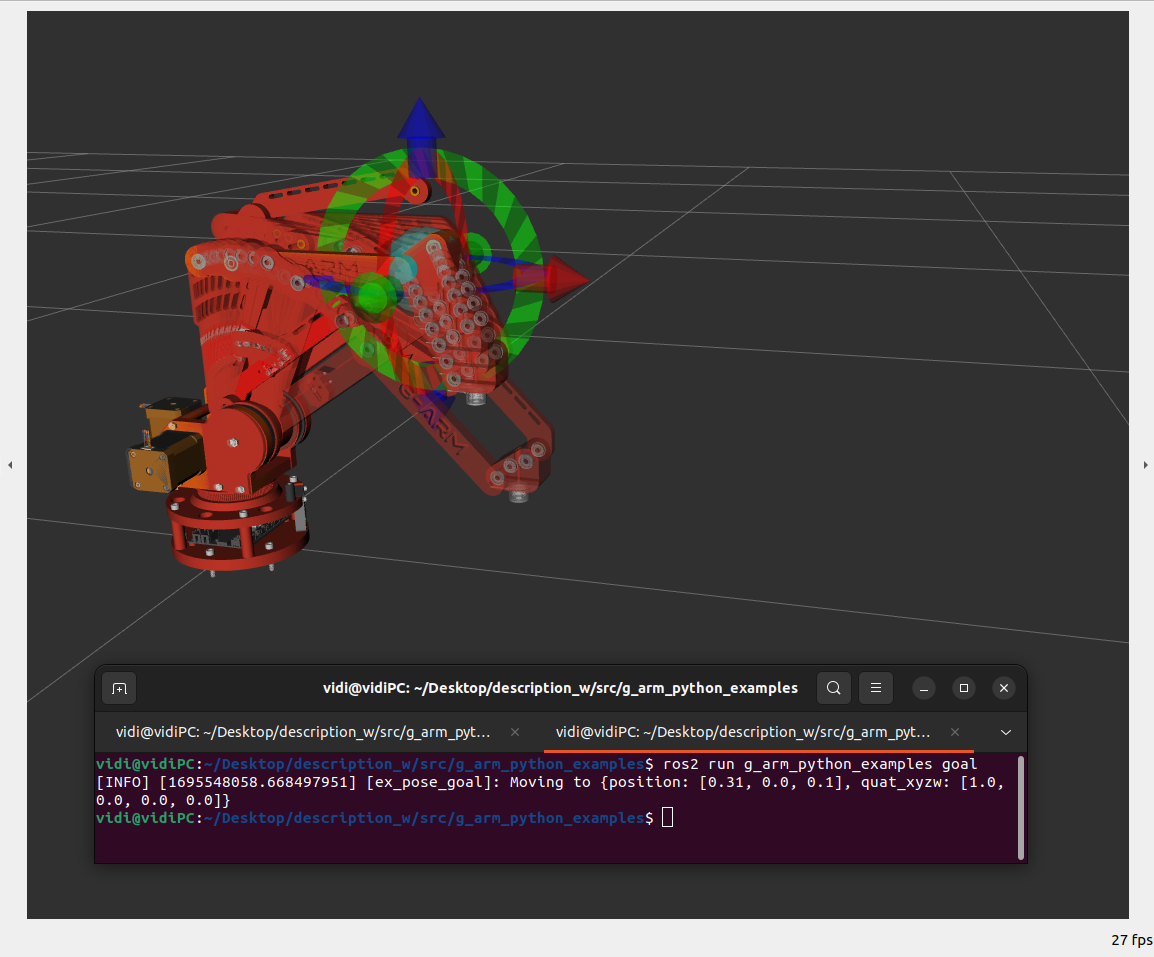
\includegraphics[width=14cm]{figs/examples_goal.png}
    \end{center}
    \caption{Recorrido del robot de la posición Home hasta el punto (0.3, 0.0, 0.1)}
\label{fig:goal}
\end{figure}

\newpage


Por otro lado, para demostrar su uso en trayectorias, se ha programado un fichero en Python con varias funciones las cuales devuelven una lista de vértices de diferentes 
figuras: corazón, cuadrado, triángulo y círculo. Estos vértices han sido utilizado como puntos de paso en el fichero de 
ejemplo\footnote{\url{https://github.com/RoboticsURJC/tfg-vperez/blob/main/src/software/g\_arm\_python_examples/g\_arm_python\_examples/trajectory.py}} para 
dibujar las diferentes figuras de prueba en el plano XY a una cierta altura en Z. Para ver su funcionamiento, ejecutamos:
\begin{verbatim}
    # Ejecutamos esto para lanzar Rviz y los nodos necesarios de MoveIt2
    ros2 launch g_arm_moveit2 show_end_effector_travel.launch 
    # Para trazar un corazón (figura por defecto)
    ros2 run g_arm_python_examples trajectory
\end{verbatim}

En la Figura \ref{fig:trayectorias} se puede ver las distintas trayectorias de ejemplo ejecutadas .

\begin{figure} [ht!]
    \centering  
    \subfigure[Cuadrado]{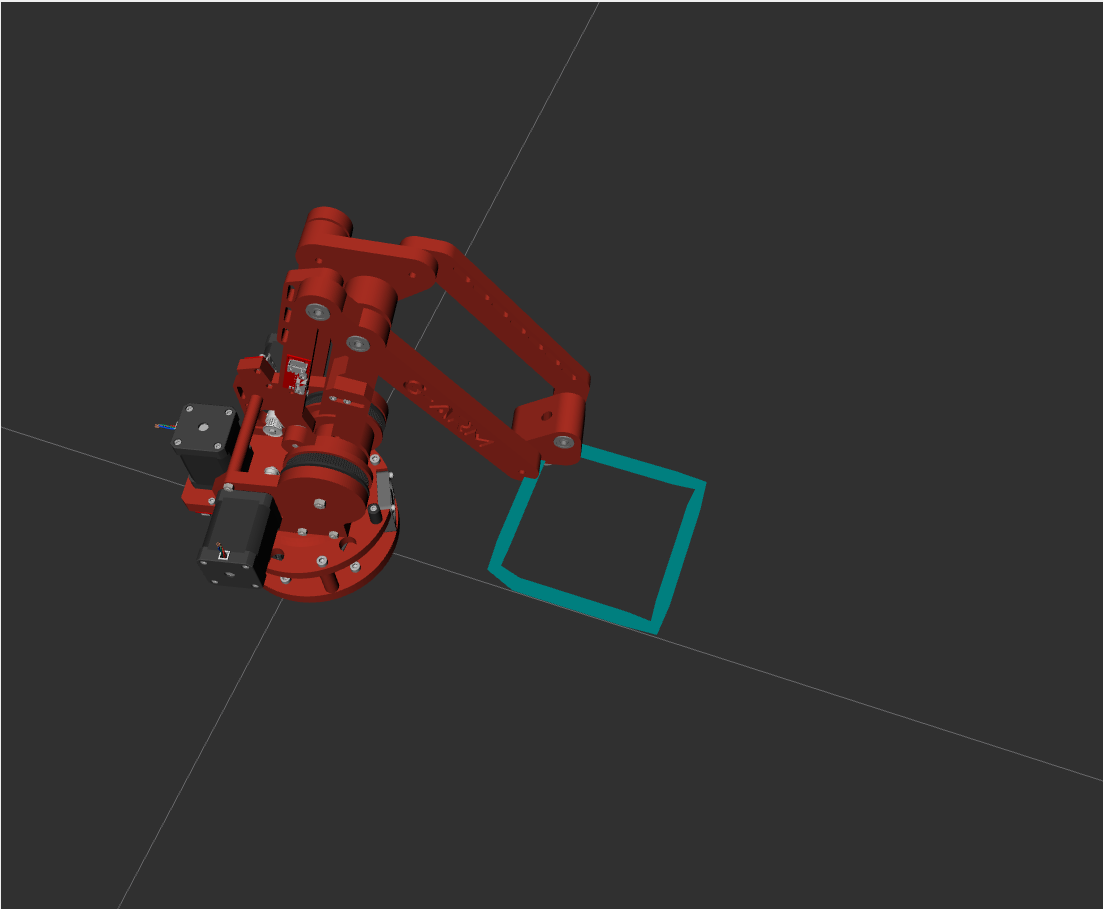
\includegraphics[width=0.4\linewidth ]{figs/square.png}}
    \hspace{2cm}
    \subfigure[Círculo]{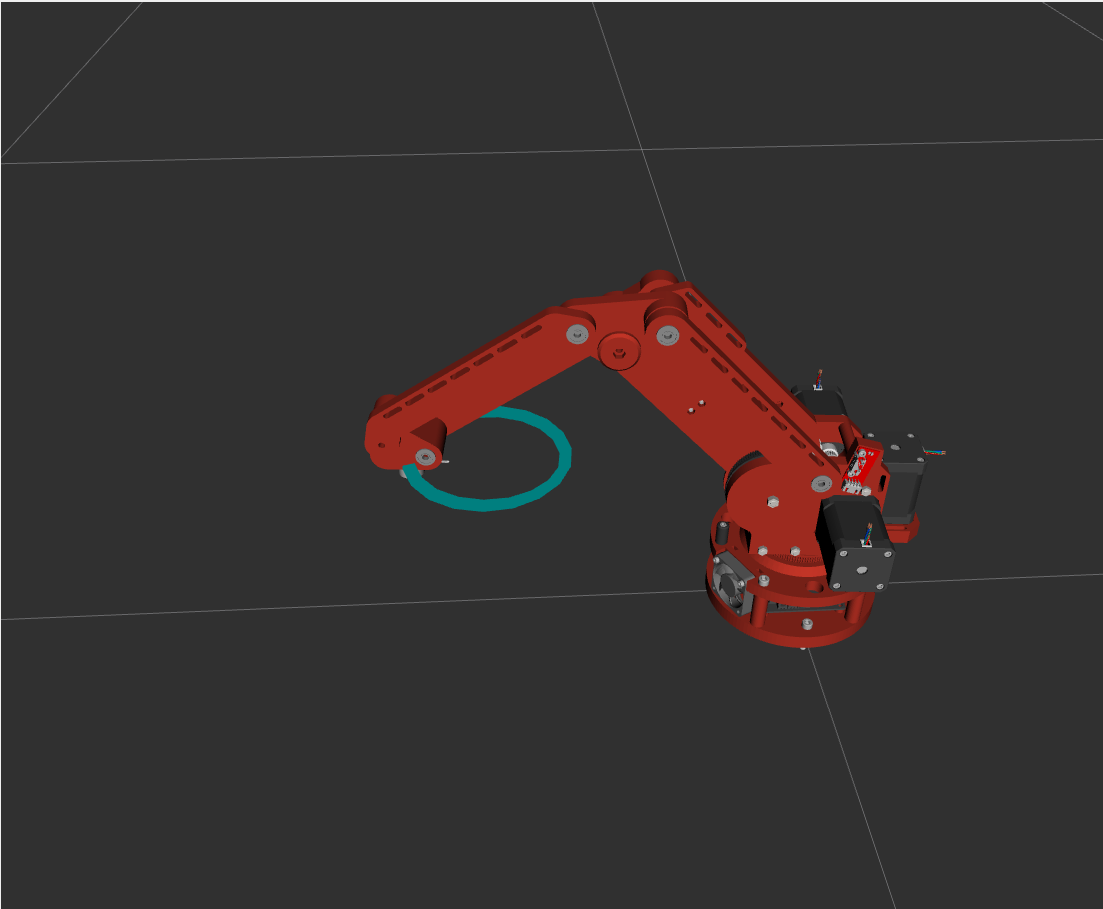
\includegraphics[width=0.4\linewidth ]{figs/circle.png}}
    \hspace{2cm}
    \subfigure[Triángulo]{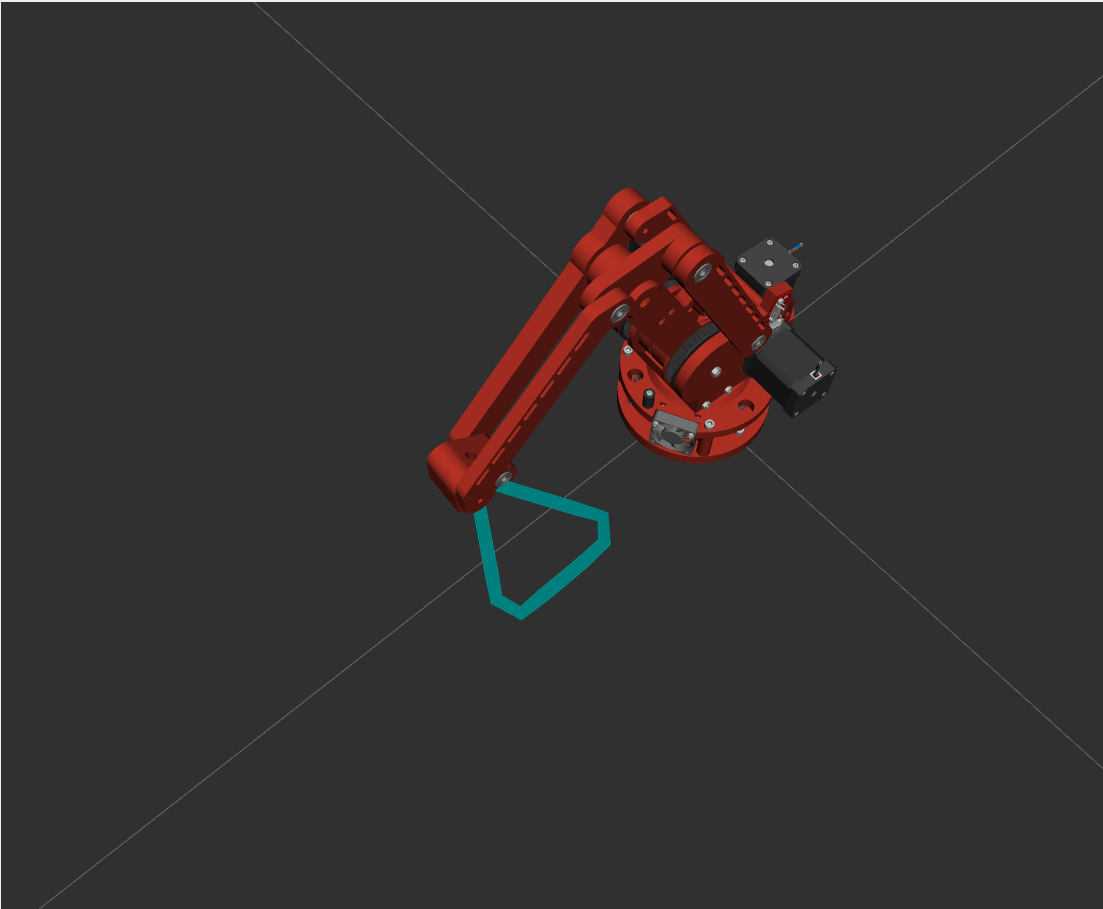
\includegraphics[width=0.4\linewidth ]{figs/triangle.png}}
    \hspace{2cm}
    \subfigure[Corazón]{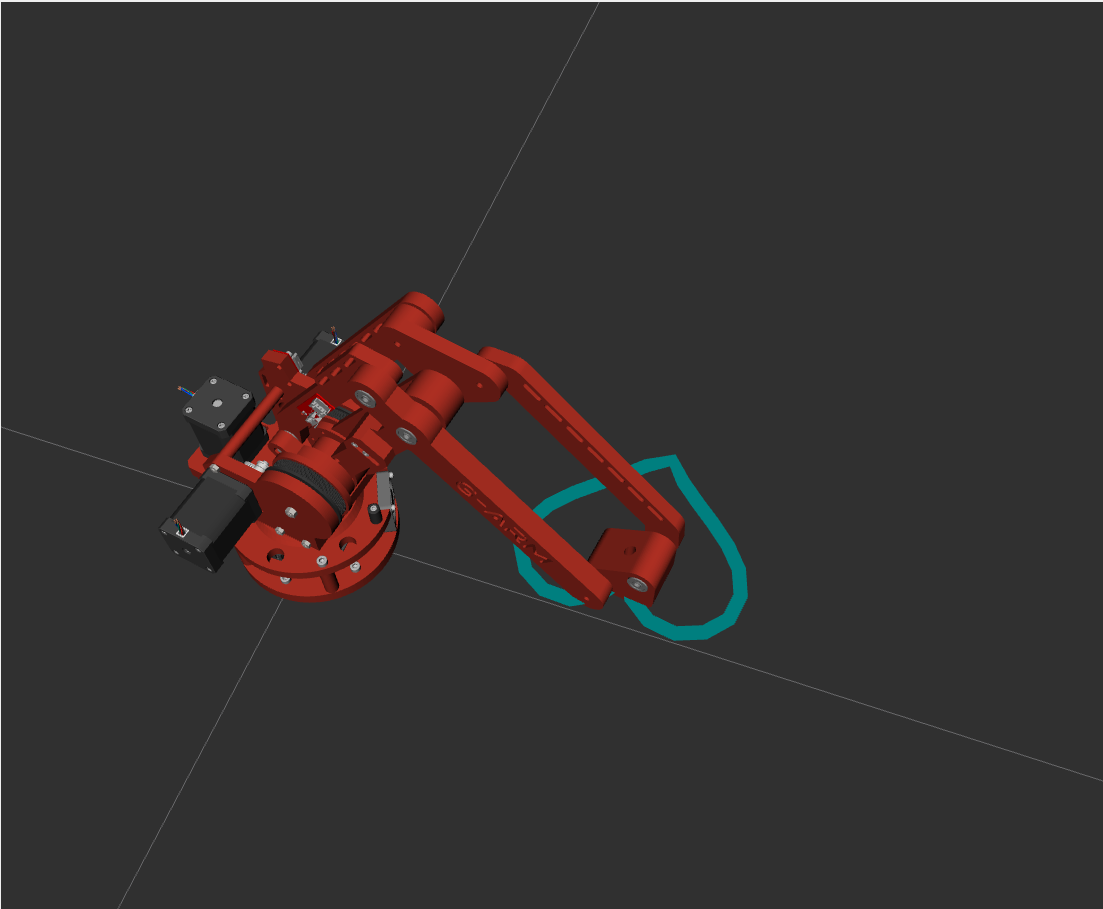
\includegraphics[width=0.4\linewidth ]{figs/heart.png}}
    \caption{Trayectorias realizadas}
    \label{fig:trayectorias}
\end{figure}\ 
\newpage
Para visualizar el recorrido de un determinado eslabón se debe de activar la opción Show Trail de RobotModel. En este caso interesa activar la 
del extremo del robot, como se puede ver en la Figura \ref{fig:activarTrail}.
\begin{figure} [ht!]
    \begin{center}
        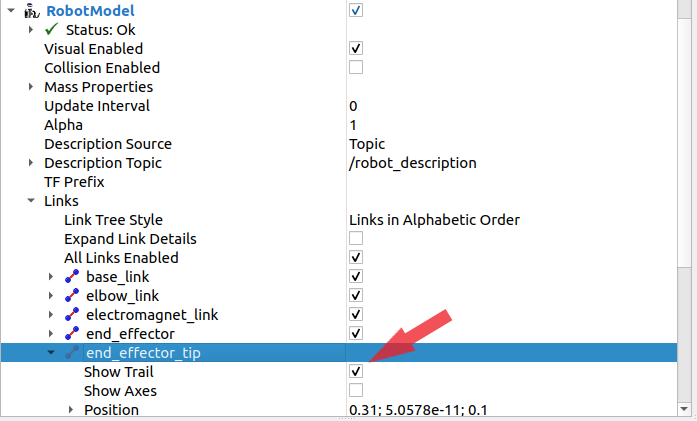
\includegraphics[width=12cm]{figs/rviz_show_trail.png}
    \end{center}
    \caption{Activación de la opción Show Trail de un link en Rviz}
\label{fig:activarTrail}
\end{figure}



Finalmente, con el objetivo de probar esto en el robot real, se ha diseñado una herramienta nueva (Figura \ref{fig:pen_tool}). Se trata de un porta lápices que utiliza la 
flexión del PLA para acoplar el lápiz al extremo del robot de una forma robusta y sin holguras pero a su vez flexible.
\begin{figure} [ht!]
    \centering  
    \subfigure[Vista lateral]{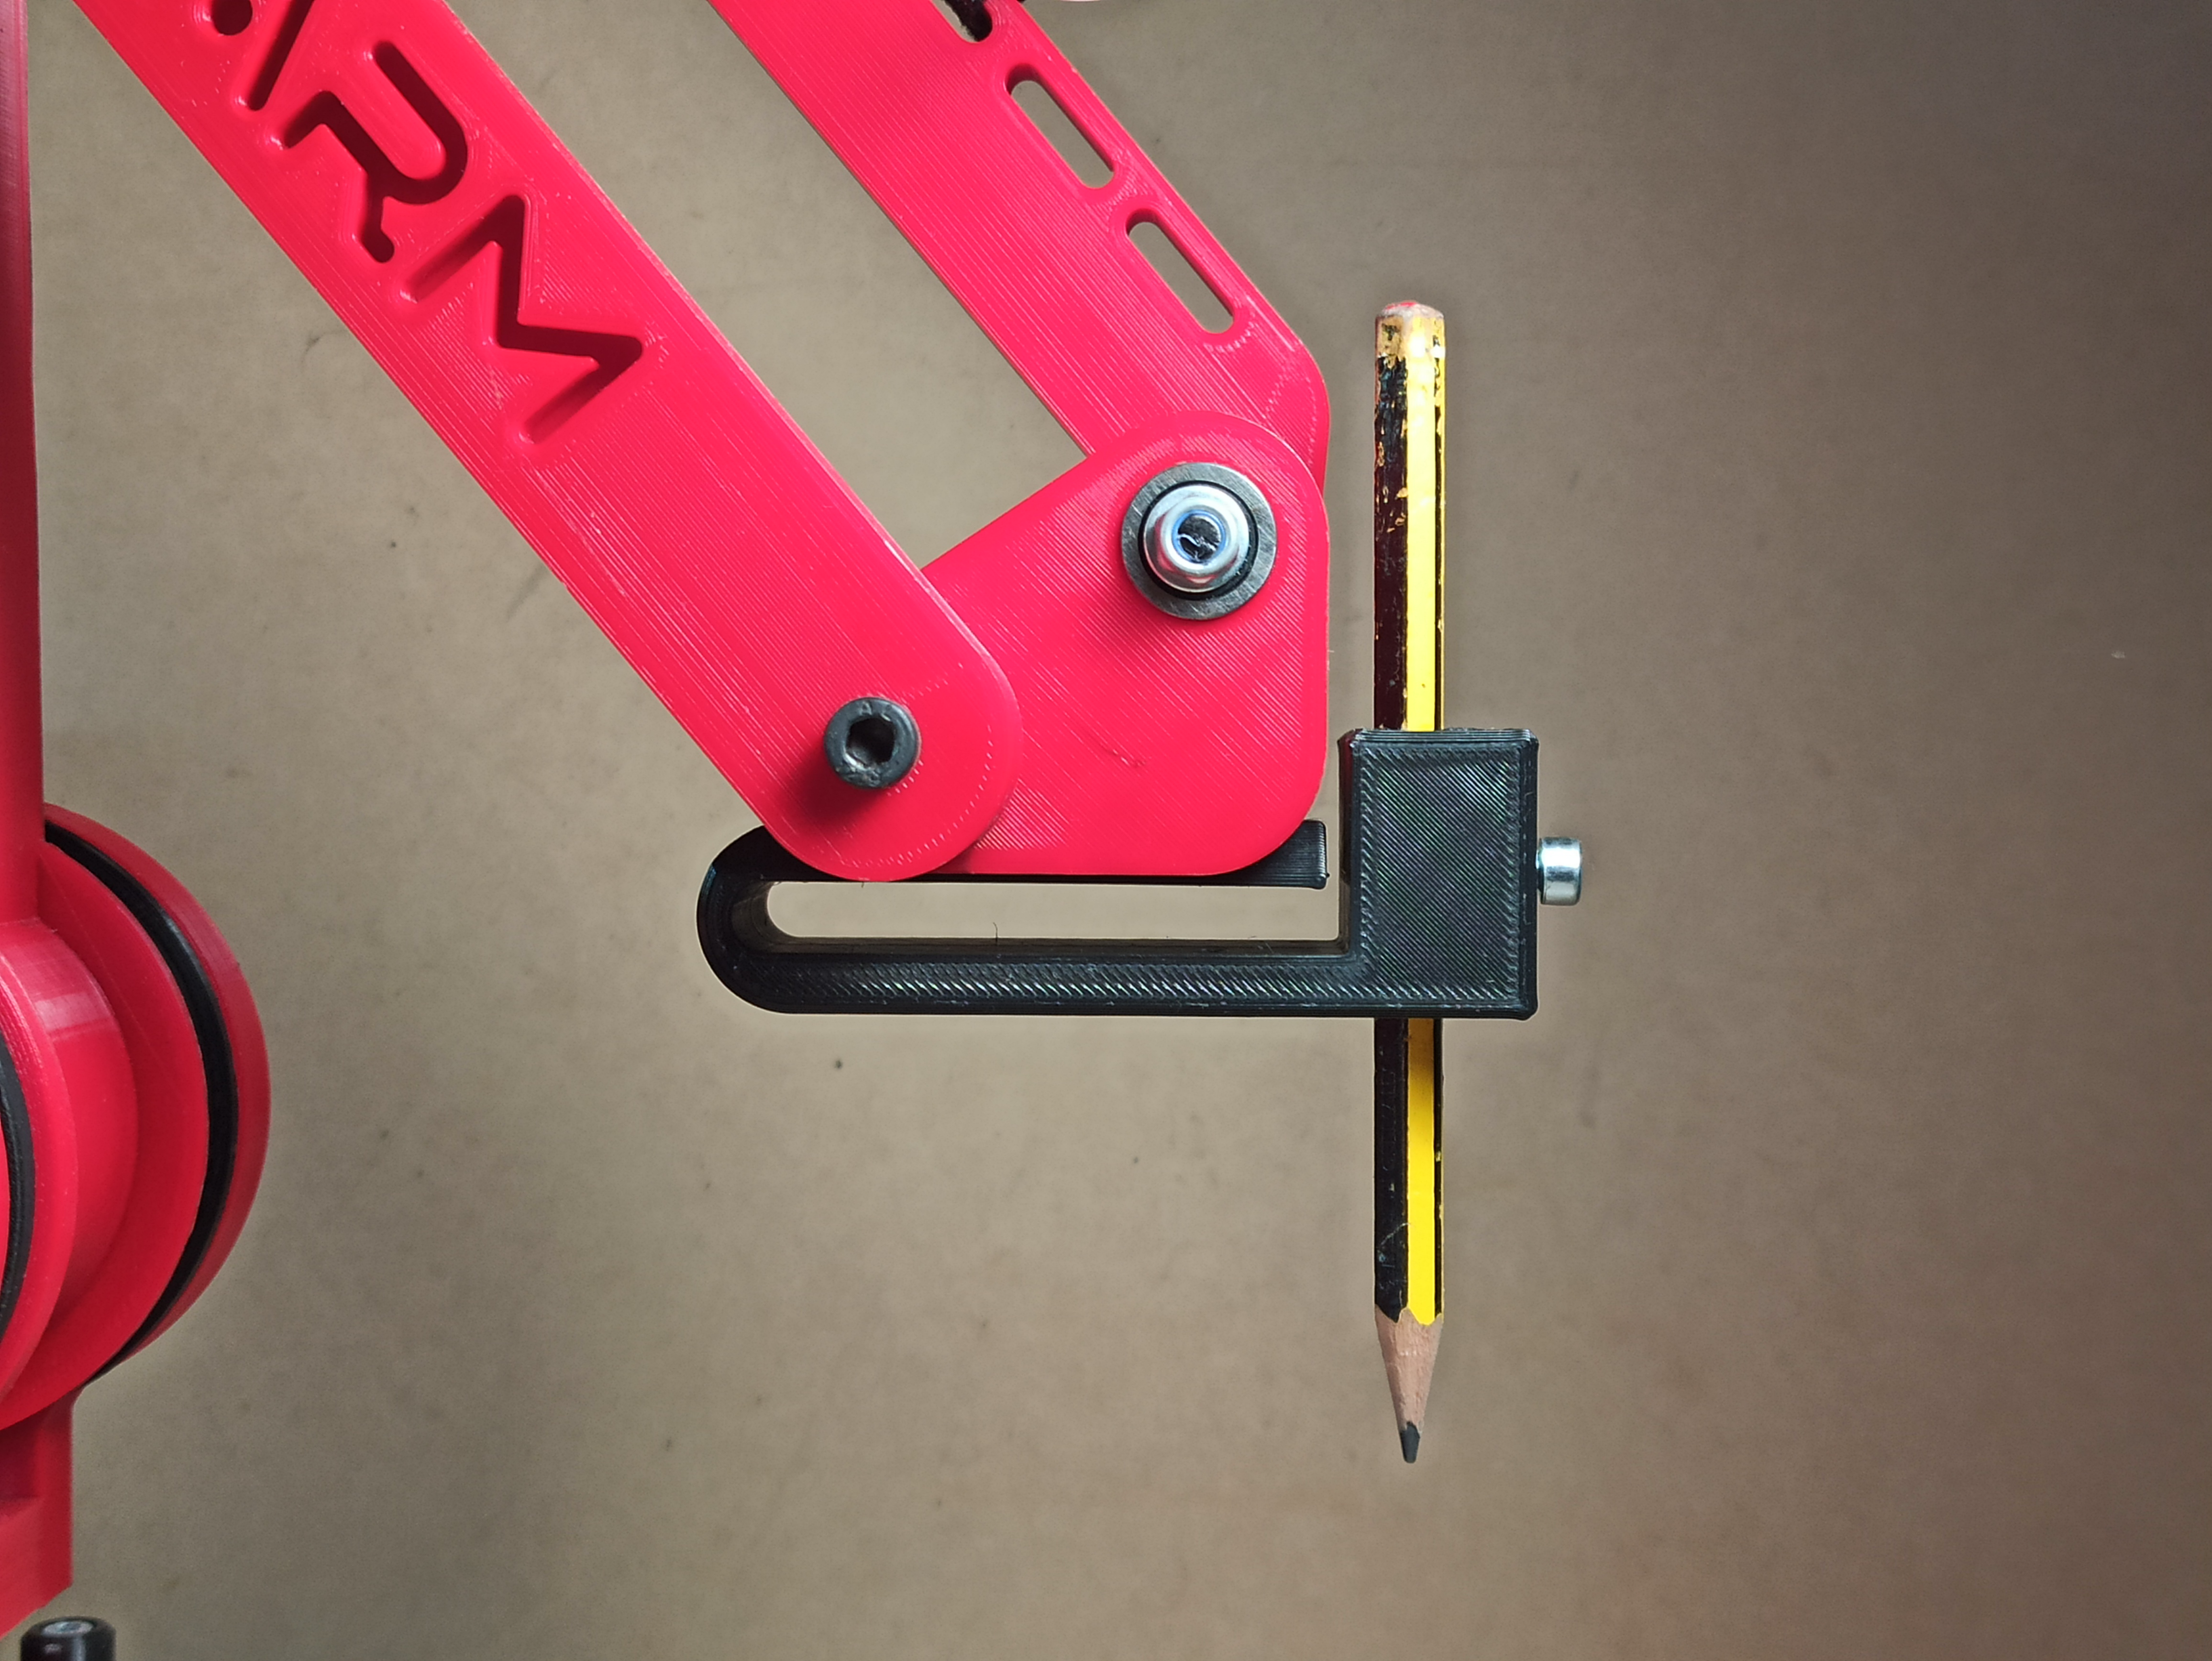
\includegraphics[width=0.45\linewidth ]{figs/pen_tool.jpg}}
    \hspace{1cm}
    \subfigure[Vista completa]{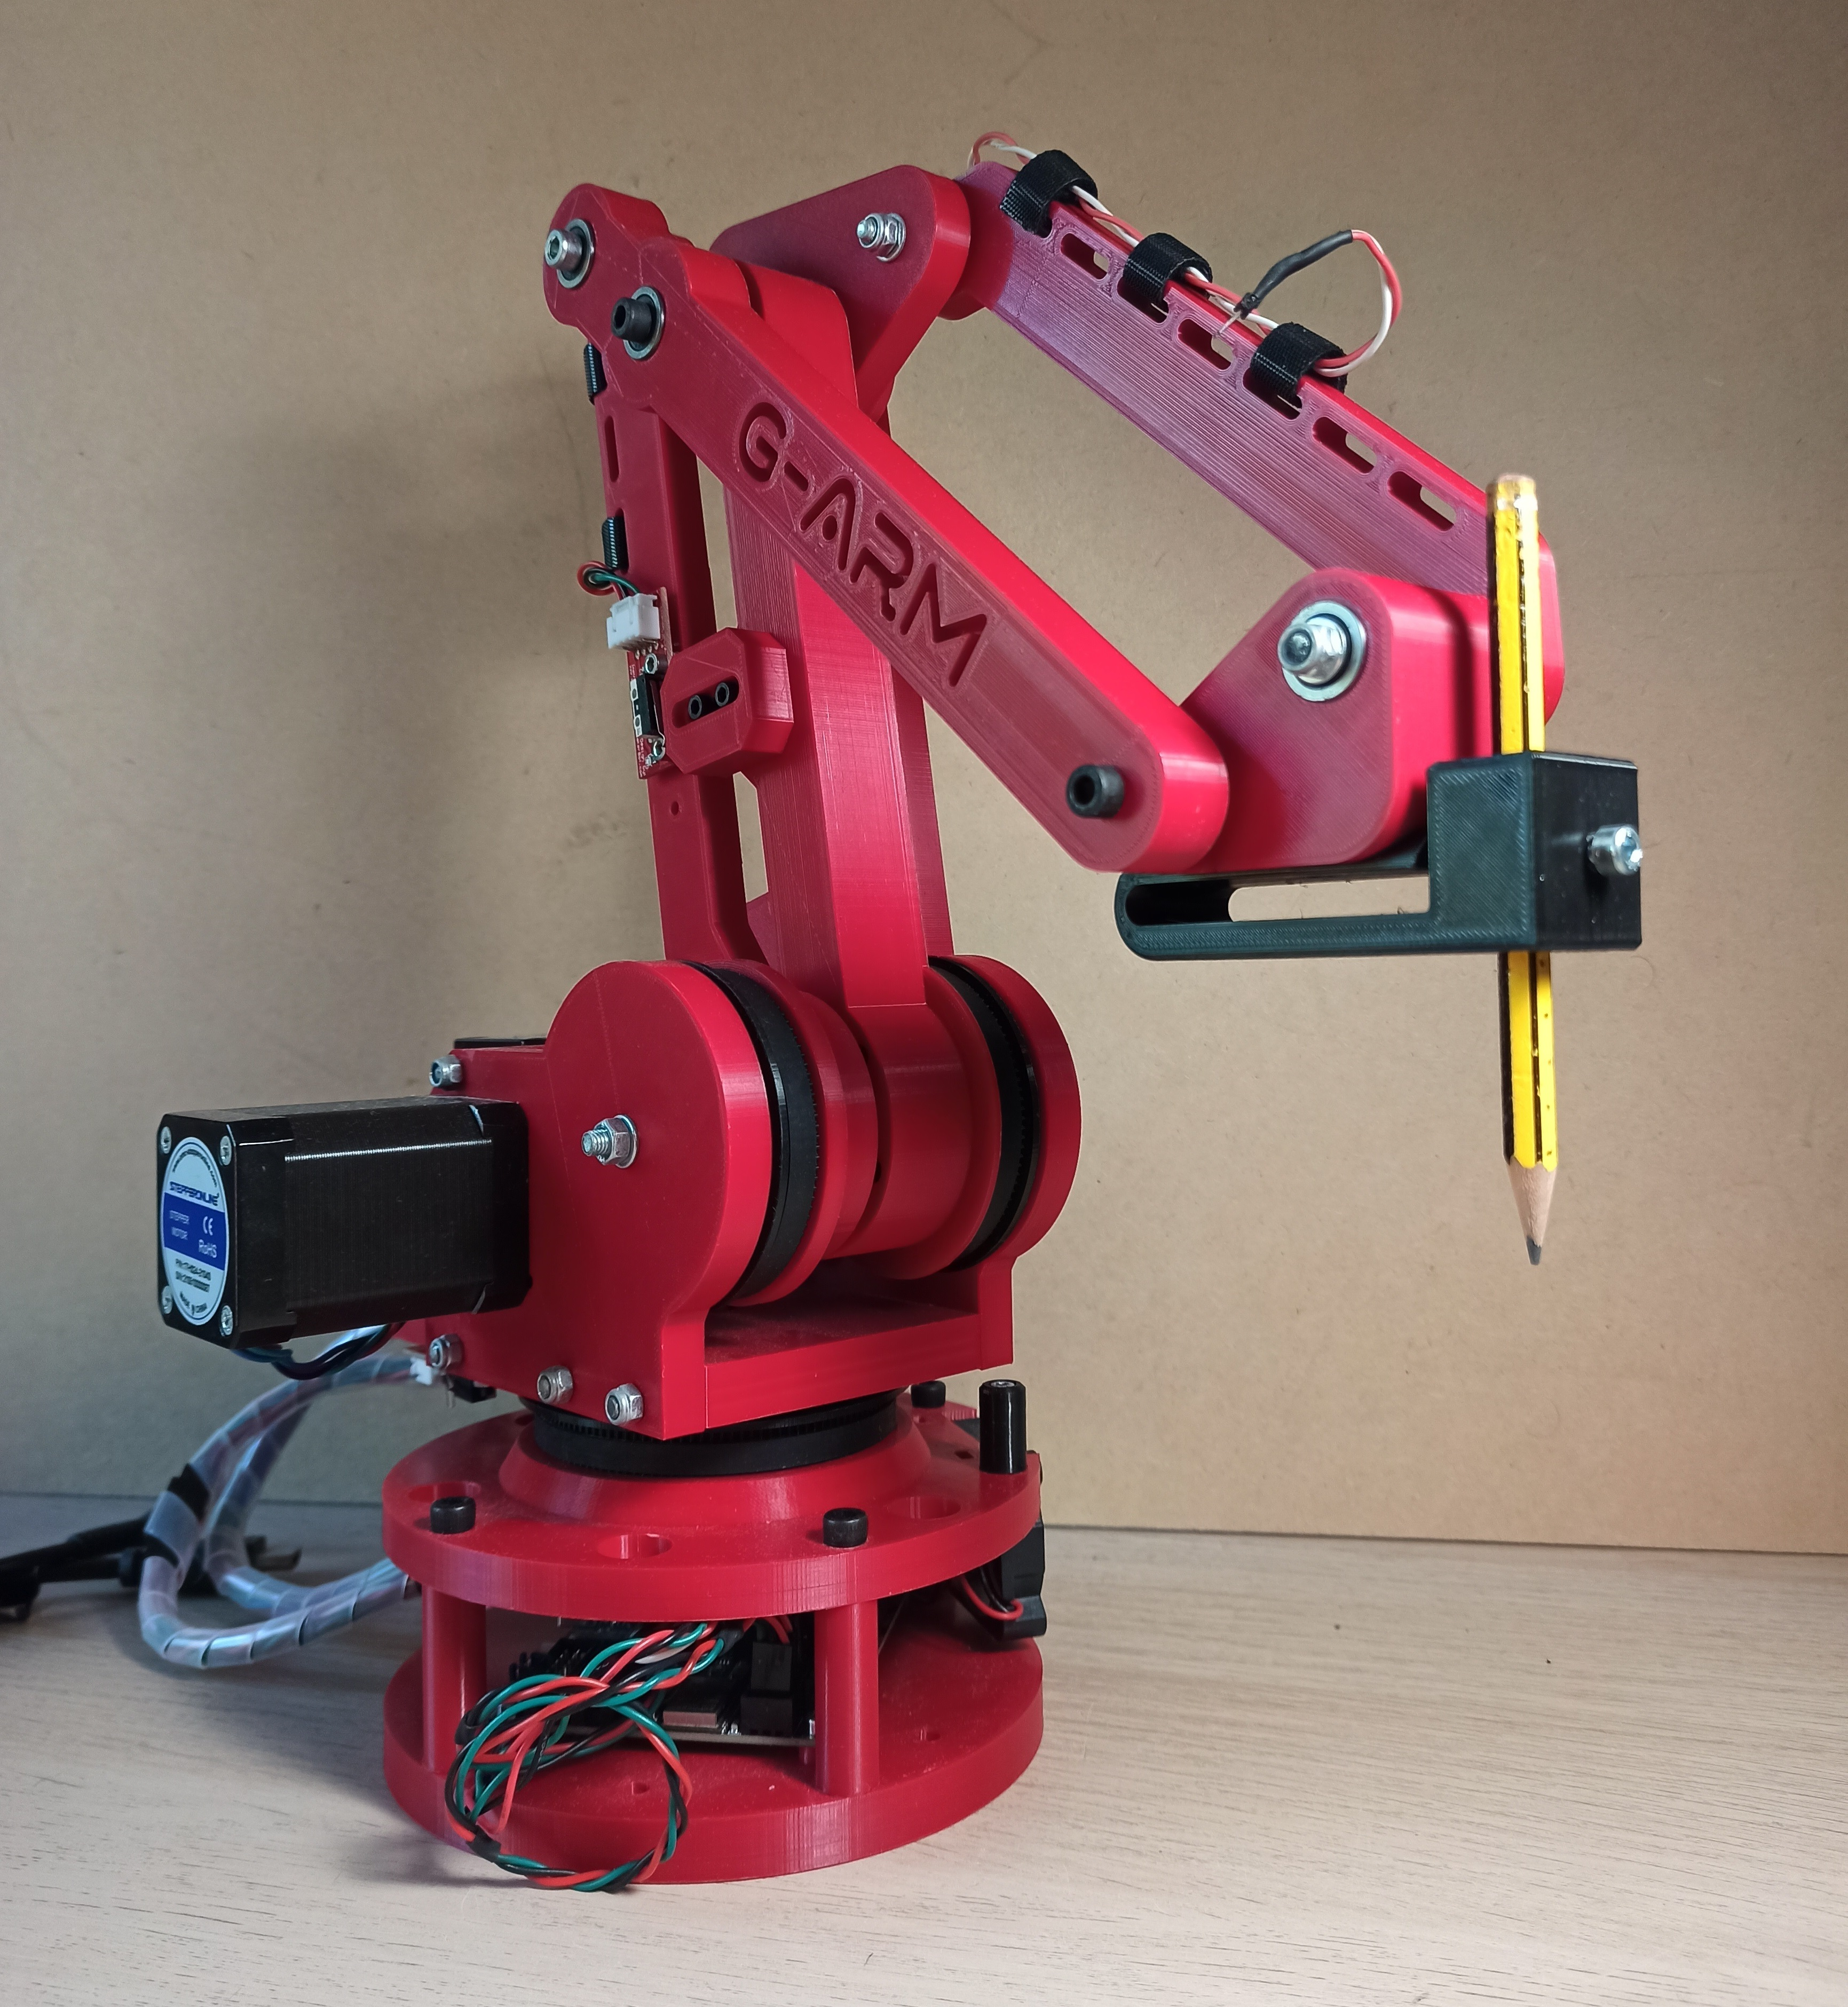
\includegraphics[width=0.45\linewidth ]{figs/robot_with_pen.jpg}}
    \caption{Herramienta porta lápices}
    \label{fig:pen_tool}
\end{figure}\ 
\newpage
Se ha escogido un plano con una altura en Z igual a 10cm, ya que en este plano es capaz de alcanzar una gran cantidad de puntos. En él se ha dispuesto 
una base plana y un folio en el que se ha dibujado la figura más compleja del ejemplo, el corazón. El resultado de todo el dibujo puede verse en el siguiente 
vídeo. Adicionalmente, en la Figura \ref{fig:real_draw} se muestra algunas imágenes extraídas del propio vídeo\footnote{\url{https://youtube.com/shorts/3rwK_FV3eSs}}.
\begin{figure} [ht!]
    \centering  
    \subfigure[Durante la trayectoria]{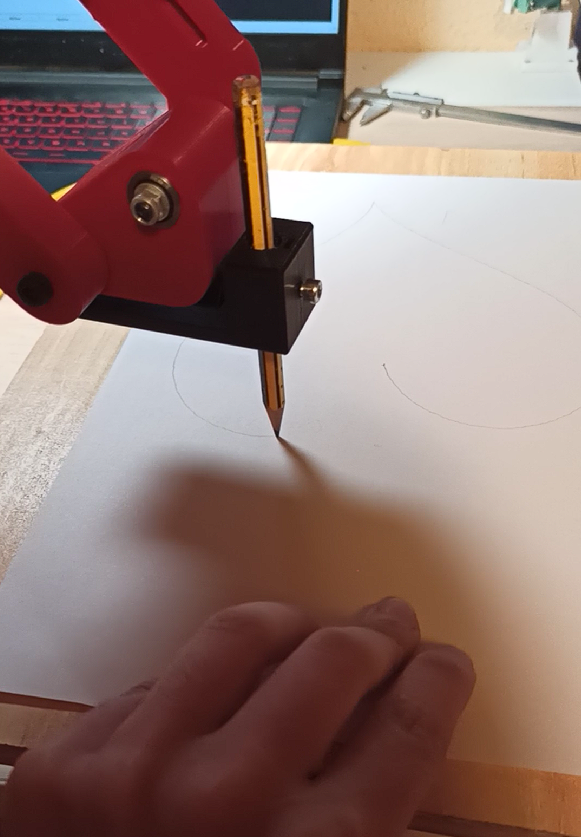
\includegraphics[width=0.45\linewidth ]{figs/drawing.png}}
    \hspace{1cm}
    \subfigure[Resultado final]{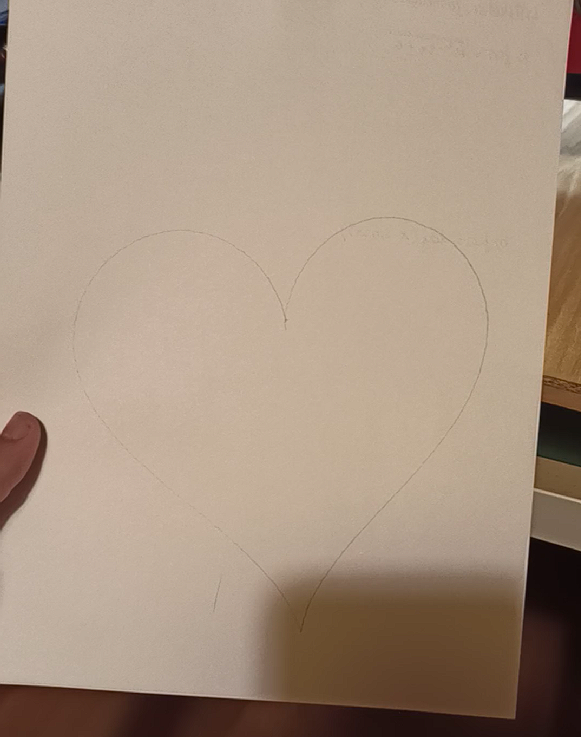
\includegraphics[width=0.45\linewidth ]{figs/drawing_result.png}}
    \caption{Prueba en el robot real}
    \label{fig:real_draw}
\end{figure}\ 

Como se puede ver el resultado es exacto y vistoso, por lo que puede ser utilizado para realizar todo tipo de trayectorias asegurando exactidud y precisión.
